\section{A New Design for Building Secure Systems}
\label{sec.design}

Once we had verified our hypothesis that ``commonly used kernel paths'' contain fewer bugs (\S{\ref{sec.metric}}), 
we set out to use this idea to build a secure system that can effectively mitigate 
the problem of kernel bug exploitation. The key idea of our design is that the system 
should have a very small TCB that accesses only the safe portion of the kernel, 
which we previously determined was the commonly used kernel paths. 
Complex and dangerous system functions, which may access the risky portion of the kernel, 
are reimplemented by our own code within a sandbox. 
Therefore, any bugs or failures within the implementation of those complex system functions 
will be contained by the sandbox, and will not have the chance to reach 
and trigger risky portions of the kernel. Thus, we call it a ``safe-reimplementation'' design.

\begin{figure}[h]
\centering
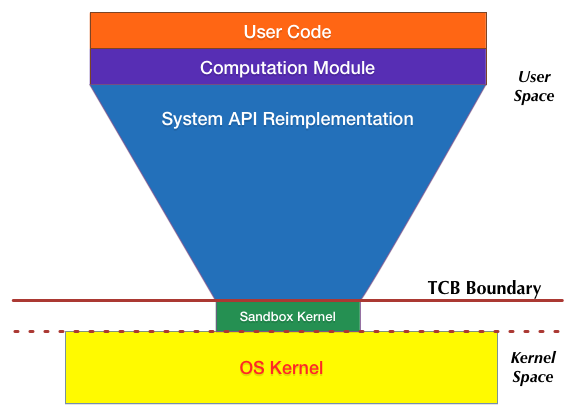
\includegraphics[width=1.0\columnwidth]{diagram/lind_secure_design.png}
\caption{The Idealized ``Safe-Reimplementation'' Design}
\label{fig:design}
\end{figure}

\subsection{Architecture}

To execute untrusted applications in a safe manner that will not trigger bugs 
in the underlying OS kernel and cause damage to other parts of the system, 
our design intent is to build a sandbox system that can provide isolation and 
containment for any improper operations in the programs. 
One approach to building such a system is to place it entirely in the user space, 
and to only have a small sandbox kernel with restricted access to the OS kernel (Figure \ref{fig:design}). 
This approach has advantages over other approaches that require modifications to 
the OS kernel, because it avoids the risk of threat escalation. If modified modules 
are inside the OS kernel, they have kernel privileges that could allow attacks on the underlying OS, 
as well as applications run on top of it. 

There are two main components in our design of a secure sandbox system (Figure \ref{fig:design}). 
The first is a computation module, which performs functions like type checking, object creation, 
and garbage collection. The second is a system API that serves requests to access the OS kernel. 
Those two components should work together to complete the requirements of running user code. 
To run this code in our sandbox system, we first invoke the computation module to perform its operations. 
Whenever there are system call requests, 
the computation module will direct those requests to our system API. 
The system API will respond to the system call requests and return results to the user code if the requests are granted. 

\subsubsection{The Computation Module}

Our secure system should be able to support and run legacy applications, 
and execute binary code compiled from unmodified source code on popular hardware architecture, 
like x86 architecture. Providing an execution environment that can run unmodified source code is 
the main responsibility of the computation module. The key security issue of executing system calls 
without triggering OS kernel bugs is left to the system API module.

\subsubsection{The System API Module}

The system API module is the core of our sandbox system. It is comprised of two parts, 
a system API safe reimplementation, and the sandbox kernel. 
The sandbox kernel is the TCB of our system, which needs to be secure and bug-free. 
Thus, in our design, we require that the sandbox kernel be small, containing not more than 10K LOC. 
It should have a set of capabilities that enable the construction of essential and more complicated functions. 
For example, the sandbox kernel capabilities should include basic functions for network, 
file system I/O, lock, thread, and namespace. It also needs to have access to the OS kernel through system calls. 
In developing our design, we leveraged our verified hypothesis that commonly used kernel paths contain fewer bugs. 
Thus, the system calls we allow in our sandbox kernel are common calls, like file open, read, write, and close. 
Furthermore, the set of arguments used for each call is also highly restricted. 

The system API safe reimplementation is a set of more complicated system calls 
that are constructed from our sandbox kernel. it should include reconstruction of 
complex system functions like many in the file system API. 
We reimplemented those system calls because we did not want user code 
to have direct access to the underlying OS kernel. 
Therefore, our reimplementation layer serves as a mediator between the user code 
and the OS kernel. In our design, the reimplementation is safe 
because the reconstruction of system calls is isolated in a sandbox. 
This can be done by choosing a memory-safe programming language to write code for the reimplementation. 
With this design, even if there are bugs in the function reimplementation, 
they cannot escape from the sandbox and will not reach the underlying OS kernel. 

Here is an example of how this reimplementation would work with the symbolic link function. 
If there is a bug in this function, our safe reimplementation will not rely on the kernel code paths for symbolic links. 
Instead, our sandbox system will implement the (incorrect) buggy behavior, but do so within the sandbox. 
Since the reimplementation code does not have privileged access to the system as the OS kernel does, 
this will not result in a security issue. The usual outcome of a bug in this case is simply that the application will fail.

With the computation module and the system API module, unmodified user code is able to run on top of our designed system. 
It is important to note that our design does not rely on any specific technique or tool. 
To implement the computation module and the system API module in our design, 
it is possible to choose from several different techniques that fit well with the users' specific needs or requirements.

This general system design was implemented as a prototype secure system called Lind. 
In the next section, we provide a detailed description of Lind.
